% ======================= Pre-Amble =========================
      
%Format
\documentclass[11pt, oneside]{article}   	% use "amsart" instead of "article" for AMSLaTeX format 
                     						%imports package {article} and specify option(s) [11pt, oneside]
\usepackage{geometry}                		% See geometry.pdf to learn the layout options. There are lots. 
    \geometry{letterpaper}                   		% ... or a4paper or a5paper or ... 
    %\geometry{landscape}                		% Activate for rotated page geometry

\usepackage[parfill]{parskip}    		        % Activate to begin paragraphs with an empty line rather than an indent

    %Colours
    \usepackage{graphicx, subcaption}
    \usepackage[usenames, dvipsnames]{color}     % font colour:    \textcolor{<colour>}{text}
          									%highlight text:  \colorbox{<color>}{text}
    \usepackage{soul}						%highlight text: \hl{}     %only  yellow								
    									%list of colours: https://www.sharelatex.com/learn/Using_colours_in_LaTeX
    									
    %Bullets
    \usepackage{enumerate}     %specify type of enumeration: \being{enumerate}[<type of enumeration>]
    
    %Footnote Spacing
    \setlength{\footnotesep}{0.4cm}                  %specify spacing b/w footnotes
    \setlength{\skip\footins}{0.6cm}                    % space b/w footnotes and textbody


%Mattematics
    %American Mathematics Society packages
    \usepackage{amsmath}	   %math
    \usepackage{amssymb}       %symbols
    \usepackage{amsthm}          %theorems

    %QED
    \newcommand*{\QEDA}{\hfill\ensuremath{\blacksquare}}         %make qed filled square:    \QEDA
    \newcommand*{\QEDB}{\hfill\ensuremath{\square}}               %make qed empty square: \QEDB 
    
    \renewcommand\qedsymbol{\ensuremath{\blacksquare}}		%Proof environment


%Figures
\usepackage{caption}
\captionsetup[figure]{labelfont=bf}    %make figure labels boldface
\captionsetup[table]{labelfont=bf}     %make table labels boldface

\usepackage[hidelinks]{hyperref}                % Allows for clickable references

    %Tables
    \usepackage[none]{hyphenat}                    % Stops breaking-up words in a table (i.e. no hyphens)                                                             
    
    \usepackage{array}   
        \newcolumntype{x}[1]{>{\centering\let\newline\\\arraybackslash\hspace{0pt}}p{#1}}       %center fixed column width: x{<len>}                      
        \newcolumntype{$}{>{\global\let\currentrowstyle\relax}}                                                   % let us apply things (e.g. bold/italicize) to entire row            
        \newcolumntype{^}{>{\currentrowstyle}}
        \newcommand{\rowstyle}[1]{\gdef\currentrowstyle{#1} #1\ignorespaces}
    
    %Images
    \graphicspath{ {images/} }                          %directory that your images are located in within your current directory
    
    %Diagrams
    \usepackage[latin1]{inputenc}
    \usepackage{tikz}
    	\tikzset{line/.style={-latex'}}
        \usepackage{tkz-berge}
        \usetikzlibrary{shapes,arrows}
        \usetikzlibrary{patterns}			%Specify colours of stuff (e.g. vertices): 
        								%	-> set style: \tikzset{VertexStyle/.append style = {minimum size = 8pt, inner sep = 0pt}} 
								%	-> change individual vertices: \AddVertexColor{white}{1,2} 


%Bibliography
\usepackage[numbers,sort&compress]{natbib}   %for multiple references: sorts  (i.e. [1,2] NOT [2, 1] )
                                           				  %                                     compresses (i.e. [1-3] )
\usepackage[nottoc]{tocbibind}                            %add bibliography to table of contents


%Miscellaneous
\usepackage{dirtytalk}    %quotations: use \say  


%================== Header & Footer =========================
\usepackage{fancyhdr}
\usepackage{lastpage}      %ensures you can reference LastPage (i.e. Page 2 of 10)

\renewcommand{\headrulewidth}{0.4pt}		%Decorative Header line: thickness={0.4pt}
\renewcommand{\footrulewidth}{0.4pt}		%Decorative Footer line: thickness={0.4pt}

\setlength{\headheight}{13.6pt} 		%space b/w top of page & header
\setlength{\headsep}{0.3in}		%space b/w page header and body

%Make Header & Footer    
\pagestyle{fancy}
    \lhead{Stephanie Knill} 		% controls the left corner of the header
    \chead{} 					% controls the center of the header
    \rhead{} 					% controls the right corner of the header
    \lfoot{} 					% controls the left corner of the footer
    \cfoot{Page~\thepage\ of \pageref{LastPage}} 				% controls the center of the footer
    												%Page~\thepage\  if just want Page x
    \rfoot{}			 		% controls the right corner of the footer

% =============================== Document ===================================
\begin{document}

% Title Page
\title{MATH 442 --- Assignment 7 \\
\line(1,0){360} \\              %(slope x, y){length of line}
}
\author{
Stephanie Knill \\
54882113 \\
Due: March 3, 2016}

\date{}                   % Activate:  display a given date (e.g. {August 4} ) or no date (empty {} )
                                    %No activate: display current date
\maketitle

%\thispagestyle{empty}                   %Remove header from this (first) page. Change empty -> plain to keep numbering
%								-> Doesn't matter in this case (b/c title page)
%\cleardoublepage


% ================= Questions ================

\section*{Question 37}

Multiplying the colour assignments of the vertices in Figure \ref{Graph1} gives us the chromatic polynomial for our graph $G$:
	$$P_G(k) = k \cdot (k-1)^2\cdot (k-2)^2$$
By similar procedure, we have that the chromatic number of Graph $G'$ (Figure \ref{Graph2}) is
	$$P_{G'}(k) = k \cdot (k-1)^3 \cdot (k-2)$$
	
	\begin{figure}[h]           
            \centering
            \begin{subfigure}[b]{0.45\columnwidth}
            	\centering
             	 \begin{tikzpicture}[scale=0.75,transform shape]
        		
        		\GraphInit[vstyle=Classic]					%Make vertice labels outside it
        		%\SetVertexNoLabel							%No vertice labels
        		\tikzset{VertexStyle/.append style = {fill=black, circle}}		%Set vertex style        		
			\Vertex [x=0,y=0, L= $k-1$]{1}
			\Vertex [x=3, y=0, L=$k-2$]{2}
			\Vertex [x=3, y=3, L=$k-2$]{3}
			\Vertex [x=0, y=3, L=$k-1$]{4}
			\Vertex [x=1.5, y=5,L=$k$]{5}
        		%\AddVertexColor{white}{1,2} 					%Change individual vertex type
            
        			\path [thick] (1) edge (2);			%arrows: [line];     label: {$label}$
			\path [thick] (2) edge (3);
			\path [thick] (3) edge (4);
			\path [thick] (1) edge (4);
			\path [thick] (3) edge (5);
			\path [thick] (4) edge (5);

            	\end{tikzpicture}
            	\caption{Graph $G$}
		\label{Graph1}
            \end{subfigure}
           \begin{subfigure}[b]{0.45\columnwidth}
            	\centering
             	 \begin{tikzpicture}[scale=0.75,transform shape]
        		
        		\GraphInit[vstyle=Classic]					%Make vertice labels outside it
        		%\SetVertexNoLabel							%No vertice labels
        		\tikzset{VertexStyle/.append style = {rectangle}}		%Set vertex style        		
			\Vertex [x=0,y=0, L=$k$]{1}
			\Vertex [x=2, y=0, L=$k-1$]{2}
			\Vertex [x=4, y=0, L=$k-1$]{3}
			\Vertex [x=6, y=0, L=$k-1$]{4}
			\Vertex [x=3, y=2, L=$k-2$]{5}
        		%\AddVertexColor{white}{1,2} 					%Change individual vertex type
            
        			\path [thick] (1) edge (2);			%arrows: [line];     label: {$label}$
			\path [thick] (2) edge (3);
			\path [thick] (3) edge (4);
			\path [thick] (2) edge (5);
			\path [thick] (3) edge (5);

            	\end{tikzpicture}
            	\caption{Graph $G'$}
		\label{Graph2}
            \end{subfigure}
           
            \caption{Graphs $G$ and $G'$ where each vertex is labelled by the number of ways it can be coloured $k$ colours.}
            \label{polynomials}
        \end{figure}



\section*{Question 38}

For the complete graph $K_n$, where $n \geq 2$, we have that each vertex is adjacent to every other vertex, thereby giving a chromatic number of
	$$\chi(K_n) = n$$

If we remove an edge $e$ joining vertices $v_1$ and $v_2$ from our complete graph, then these vertices are no longer adjacent in our new graph $K_n - e$. Since we can now colour $v_1$ and $v_2$ the same colour, the chromatic number of $K_n - e$ is equivalent to the chromatic number of a complete graph of $n-1$ vertices:
	\begin{align*}
		\chi(K_n - e) & = \chi(K_{n-1}) \\
		& = n-1
	\end{align*}


\section*{Question 39}

\textbf{Conjecture:} The chromatic polynomial of any \textit{tree} (a connected graph that contains no cycles) with $n$ vertices is $k(k-1)^{n-1}$.

\begin{proof}
We will proceed by strong induction on the number of vertices $n$.

\textbf{Base Case:} $n=1$

Here we have a null graph of 1 vertex, which has a chromatic polynomial of $k^n = k^1 = k$. Using our formula for the chromatic polynomial of a tree with $n=1$ vertices likewise gives us
	\begin{align*}
		P_G(k) & = k(k-1)^{n-1} \\
		& = k(k-1)^0 \\
		& = k
	\end{align*}

\textbf{Induction Step}: assume that all trees with up to $n-1$ vertices has a chromatic polynomial of $k(k-1)^{n-1}$.

For our tree of $n$ vertices, we know there must be at least one vertex $v$ of degree 1, otherwise there would be a cycle. Let us remove this vertex $v$. Then we are left with a graph $G'$ of $n-1$ vertices and we have
	\begin{align*}
		P_{G'}(k) & = k(k-1)^{n-2}
	\end{align*}
by our induction assumption. Adding our vertex $v$ back in, we can assign it $k-1$ possible colours. Multiplying this by the chromatic polynomial of $G'$ gives us the chromatic polynomial of the graph $G$ of $n$ vertices
	\begin{align*}
		P_{G}(k) & = P_{G'}(k) \cdot (k-1) \\
		& = k(k-1)^{n-2} \cdot (k-1) \\
		& = k(k-1)^{n-1} 
	\end{align*}
\end{proof}


\section*{Question 40}

The windmill graph $Wd(n, N)$ on $N(n ? 1) + 1$ vertices is the connected simple graph formed by taking $N$ copies of $K_n$ and joining them at a common vertex. 

\textbf{Proposition:}  The chromatic polynomial of the windmill graph $Wd(n, N)$ is $$P_{Wd(n,N)} = k \prod_{i=1}^{n-1} (k-i)^N$$

\begin{proof}
For our windmill graph, let us colour our common vertex $k$ colours.

Now let us look at each $K_n$ copy separately. Since we have already coloured one of the vertices in it, we will only examine the remaining $n-1$ vertices. Here the next vertex can be coloured $k-1$ ways, the next $k-2$ ways, ... , and the $(n-1)$ vertex $k-(n-1)$ ways. Thus the chromatic polynomial of one $K_n$ copy is
	\begin{align*}
		(k-1)(k-2)\cdot \ldots \cdot (k-(n-1)) = \prod_{i=1}^{n-1} (k-i)
	\end{align*}
However, we have $N$ copies of each of these components, so we must multiply the chromatic number of each copy by the chromatic number of all other copies.
$$\prod_{i=1}^{n-1} (k-i)^N$$
Combining this with our common vertex coloured $k$ ways gives us the chromatic polynomial of our windmill graph
 $$P_{Wd(n,N)} = k \prod_{i=1}^{n-1} (k-i)^N$$
\end{proof}



\section*{Question 41}

\emph{Proposition:} Let $G$ be a simple graph with $n$ vertices. Prove that the coefficient in $P_G(k)$ of $k^n$ is 1 and of $k^{n-1}$ is $-|E(G)|$.

\begin{proof}

We will proceed by induction on the number of edges.

\textbf{Base Case:} $e=0$

Here we have a null graph of n vertices. Thus the chromatic polynomial of the null graph $G$ of $n$ vertices is
	\begin{align*}
		P_G(k) & = k^n
	\end{align*}
Here the coefficient of $k^n$ is 1 and the coefficient of $k^{n-1}$ is $0 = - |E(G)|$.

\textbf{Induction Step}: assume the proposition holds true for less than $m$ edges, where $m>0$. Let $G$ be a graph with $m$ edges. Using the Deletion-Contraction Theorem, we will choose any edge $e$ in our graph $G$ to delete and contract, which gives us
$$P_G(k) = P_{G-e}(k) - P_{G/e}(k)$$

\emph{Coefficient of $k^n$}

Since $P_{G-e}(k)$ has less than $m$ edges, then by the induction assumption we know that the coefficient of $k^n$ in $P_{G-e}(k)$ is 1. Since we contracted an edge in $P_{G/e}(k)$, we only have $n-1$ vertices. Thus the highest degree is $k^{n-1}$, which means the coefficient of $k^n$ is 0. Taking the difference of these gives us 1, which is the coefficient of $k^n$ in $P_G(k)$

\emph{Coefficient of $k^{n-1}$}

Again, $P_{G-e}(k)$ has less than $m$ edges, so by the induction assumption the coefficient of $k^{n-1}$ in $P_{G-e}(k)$ is $- |E(G-e)|$. Similarly, since $P_{G/e}(k)$ has $n-1$ vertices the highest degree is $k^{n-1}$, which has a coefficient of 1. Taking the difference between the two gives us the coefficient of $k^{n-1}$ in $P_G(k)$:
	\begin{align*}
		- |E(G-e)| - 1 & = -(|E(G)| - 1) -1 \\
		& =  -|E(G)|
	\end{align*}

\end{proof}




%\textbf{Coefficient of $k^n$} Since this is the polynomial of highest degree, the coefficient of it is obtained by multiplying the coefficients of the $k$'s in the chromatic polynomial. Each $k$ has coefficient 1, and multiplying these $n$ times gives $k^n$ a coefficient of 1.
%
%\textbf{Coefficient of $k^{n-1}$} To generate a chromatic polynomial, let us visit each vertex and assign it $k-i$ colours, where $i$ is the number of edges that connects the current vertex with all other vertices visited. This will ensure we do neither double count nor miss any of the edges. This means the for the first vertex we assign it $k$ colours, the second vertex $k-1$ colours, and the third vertex either $k-1$ or $k-2$ depending on the connectivity of the graph, and so on until we have coloured all $n$ vertices. Preceeding in this manner we generate our chromatic polynomial
%$$P_G(k) = k(k-1)^a(k-2)^b\cdot \ldots \cdot (k-(n-1))^c$$
%where $a,b,$ and $c$ are nonnegative integers. Multiplying this out we see that the coefficient of $k^{n-1}$ is the summation of all the $i$'s. 


\section*{Question 42}

\emph{Let $G$ be a simple graph. Then the chromatic polynomial $P_G(k)$ is the product of the chromatic polynomials of its components.}

\begin{proof}
Let $G$ be a simple graph. 

\textbf{Case 1:} $G$ is connected

Since $G$ consists of 1 component, then the chromatic polynomial of this one component is the chromatic polynomial of the graph $G$.

\textbf{Case 2:} $G$ is not connected

Since $G$ is a union of disjoint components $C_1, C_2, \ldots, C_n$, then---similar to the Null Graph---no two \textit{components} are adjacent. Thus we can colour $C_1$ the chromatic polynomial of that component, $C_2$ the chromatic polynomial of that polynomial, ... , and $C_n$ the chromatic polynomial of the component. So the total number of colourings is
$$P_{C_1}(k) \cdot P_{C_2}(k) \cdot \ldots \cdot P_{C_n}(k) = P_{G}(k)$$
which is the chromatic polynomial of the graph $G$.

\end{proof}


\end{document} 